% Created 2017-02-02 Thu 19:52
% Intended LaTeX compiler: pdflatex
\documentclass[11pt]{article}
\usepackage[utf8]{inputenc}
\usepackage[T1]{fontenc}
\usepackage{graphicx}
\usepackage{grffile}
\usepackage{longtable}
\usepackage{wrapfig}
\usepackage{rotating}
\usepackage[normalem]{ulem}
\usepackage{amsmath}
\usepackage{textcomp}
\usepackage{amssymb}
\usepackage{capt-of}
\usepackage{hyperref}
\author{Jake Brawer}
\date{\today}
\title{HW 1\\\medskip
\large CPSC424}
\hypersetup{
 pdfauthor={Jake Brawer},
 pdftitle={HW 1},
 pdfkeywords={},
 pdfsubject={},
 pdfcreator={Emacs 25.1.1 (Org mode 9.0.3)}, 
 pdflang={English}}
\begin{document}

\maketitle
\newcommand*\wrapletters[1]{\wrapletters#1\@nil}
\def\wrapletters#1#2\@nil{#1\allowbreak\if&#2&\else\wr@pletters#2\@nil\fi}
\wrapletters{akjhghjerbhkjgxhdrjgkbhyxksrfihcgbwaemklcjtnhwabketrbmshrkncgaervbetjkewhbgrkjavkjdkvbkjsjkbtkgvnsetbjsrhtservjbtbjkhtvy}
\section{Building and Running the Code}
\label{sec:org328049c}

\subsection{Software and Dev. Environments}
\label{sec:orgdca71c8}

All the programming for this assignment was done in vim. This document, including the figures, were made using emacs (and gnuplot). The only module loaded used in this assignment is Langs/Intel/15.


\subsection{Running Code}
\label{sec:org56becb2}

The code for this assignment is separated amongst two directories Pr1 and Pr2. To compile all the code at once, simply run setup.sh located in the toplevel directory. To run the code on Omega for problem 1, navigate into Pr1 and run pr1.sh. Running this file (\texttt{qsub pr1.sh}) will output the text file out.txt. This file contains measurements regarding the timing of the integration function, estimates of divide operation, and the estimated value of pi.

Similarly, running pr2.sh located in Pr2 outputs a file output.txt. This file contains data relating the size of N to MFLOPS.

\section{Pr 1}
\label{sec:org1267477}

The compiler flags in group d ended up resulting more 5x performance increase (\textasciitilde{}20 secs to \textasciitilde{}3 secs). This is most likely due, in part, to the compiler unrolling the loop where the arithmetic for the integration was taking place. In fact, I had originally written this using a while loop that was not easily unrolled and got \emph{no} performance increase across the compiler flags (although my worse case then was much better than my worse case now), which I think lends support to this. 

In order to calculate the latency for divides, I created a timed two toy functions. In theory these functions only differed by the presence/absence of a single floating point divide. Taking the difference between the two functions should have in theory been useful for calculating the latency. However this difference differed wildly between compiler flag options, and in general, I got an answer < 1 cycle--an impossibility. In fact, for some compiler flag groups, the function with addition was actually faster than the function without. It's clear that in this case that the compiler was actually circumventing the divisions. One possible method of doing this is to replace the division with multiplication of the reciprocal of the divisor, as multiplying is much quicker. However, this means  

The value of \(\pi\) calculate was correct to the 7th decimal place. This allowed my to estimate \(\cos(\pi)\) correctly to 1o decimal places (-1) and \(\sin(\pi)\) to 8 (0).

\section{Pr 2}
\label{sec:org9faa643}

\begin{center}
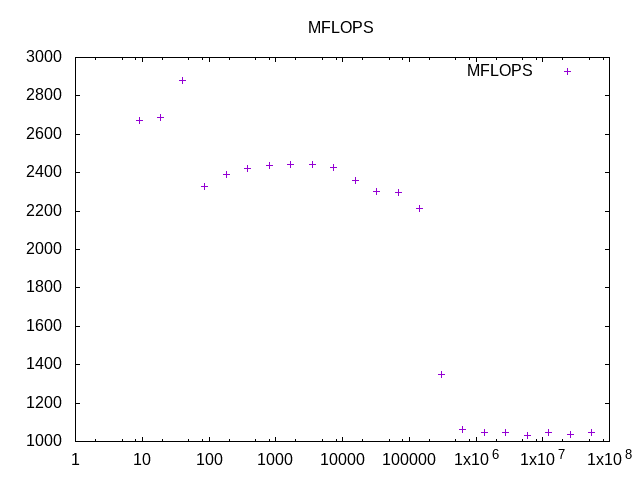
\includegraphics[width=.9\linewidth]{MFLOPS.png}
\end{center}

Above is a graph comparing array length to MFLOPS. Clearly there is a precipitous drop off in performance as N gets large. This is likely caused by the fact that large arrays wont fit in the cache. As a result, cache misses increase, resulting in more data transfer from main memory, which results in a lot of computational downtime.

\section{Env Output}
\label{sec:orgc0c8d09}
MKLROOT=/home/apps/fas/Langs/Intel/2015\(_{\text{update2}}\)/composer\(_{\text{xe}}\)\(_{\text{2015.2.164}}\)/mkl
MANPATH=/home/apps/fas/Langs/Intel/2015\(_{\text{update2}}\)/composer\(_{\text{xe}}\)\(_{\text{2015.2.164}}\)/man/en\(_{\text{US}}\):/home/apps/fas/Langs/Intel/2015\(_{\text{update2}}\)/composer\(_{\text{xe}}\)\(_{\text{2015.2.164}}\)/debugger/gdb/intel64/share/man/:/home/apps/fas/Langs/Intel/2015\(_{\text{update2}}\)/composer\(_{\text{xe}}\)\(_{\text{2015.2.164}}\)/debugger/gdb/intel64\(_{\text{mic}}\)/share/man/:/usr/share/man:/opt/moab/share/man:
GDB\(_{\text{HOST}}\)=/home/apps/fas/Langs/Intel/2015\(_{\text{update2}}\)/composer\(_{\text{xe}}\)\(_{\text{2015.2.164}}\)/debugger/gdb/intel64\(_{\text{mic}}\)/bin/gdb-ia-mic
HOSTNAME=login-0-0.local
IPPROOT=/home/apps/fas/Langs/Intel/2015\(_{\text{update2}}\)/composer\(_{\text{xe}}\)\(_{\text{2015.2.164}}\)/ipp
INTEL\(_{\text{LICENSE}}\)\(_{\text{FILE}}\)=/home/apps/fas/Langs/Intel/2015\(_{\text{update2}}\)/composer\(_{\text{xe}}\)\(_{\text{2015.2.164}}\)/licenses:/opt/intel/licenses:/home/apps/fas/Licenses/intel\(_{\text{site.lic}}\)
TERM=xterm
SHELL=/bin/bash
HISTSIZE=1000
GDBSERVER\(_{\text{MIC}}\)=/home/apps/fas/Langs/Intel/2015\(_{\text{update2}}\)/composer\(_{\text{xe}}\)\(_{\text{2015.2.164}}\)/debugger/gdb/target/mic/bin/gdbserver
SSH\(_{\text{CLIENT}}\)=172.27.41.66 41162 22
LIBRARY\(_{\text{PATH}}\)=/home/apps/fas/Langs/Intel/2015\(_{\text{update2}}\)/composer\(_{\text{xe}}\)\(_{\text{2015.2.164}}\)/ipp/../compiler/lib/intel64:/home/apps/fas/Langs/Intel/2015\(_{\text{update2}}\)/composer\(_{\text{xe}}\)\(_{\text{2015.2.164}}\)/ipp/lib/intel64:/home/apps/fas/Langs/Intel/2015\(_{\text{update2}}\)/composer\(_{\text{xe}}\)\(_{\text{2015.2.164}}\)/compiler/lib/intel64:/home/apps/fas/Langs/Intel/2015\(_{\text{update2}}\)/composer\(_{\text{xe}}\)\(_{\text{2015.2.164}}\)/mkl/lib/intel64:/home/apps/fas/Langs/Intel/2015\(_{\text{update2}}\)/composer\(_{\text{xe}}\)\(_{\text{2015.2.164}}\)/tbb/lib/intel64/gcc4.4
PERL5LIB=/opt/moab/lib/perl5
FPATH=/home/apps/fas/Langs/Intel/2015\(_{\text{update2}}\)/composer\(_{\text{xe}}\)\(_{\text{2015.2.164}}\)/mkl/include
QTDIR=/usr/lib64/qt-3.3
QTINC=/usr/lib64/qt-3.3/include
MIC\(_{\text{LD}}\)\(_{\text{LIBRARY}}\)\(_{\text{PATH}}\)=/home/apps/fas/Langs/Intel/2015\(_{\text{update2}}\)/composer\(_{\text{xe}}\)\(_{\text{2015.2.164}}\)/mpirt/lib/mic:/home/apps/fas/Langs/Intel/2015\(_{\text{update2}}\)/composer\(_{\text{xe}}\)\(_{\text{2015.2.164}}\)/ipp/lib/mic:/home/apps/fas/Langs/Intel/2015\(_{\text{update2}}\)/composer\(_{\text{xe}}\)\(_{\text{2015.2.164}}\)/compiler/lib/mic:/home/apps/fas/Langs/Intel/2015\(_{\text{update2}}\)/composer\(_{\text{xe}}\)\(_{\text{2015.2.164}}\)/mkl/lib/mic:/opt/intel/mic/coi/device-linux-release/lib:/opt/intel/mic/myo/lib:/home/apps/fas/Langs/Intel/2015\(_{\text{update2}}\)/composer\(_{\text{xe}}\)\(_{\text{2015.2.164}}\)/tbb/lib/mic
SSH\(_{\text{TTY}}\)=/dev/pts/63
ANT\(_{\text{HOME}}\)=/opt/rocks
USER=jnb37
LD\(_{\text{LIBRARY}}\)\(_{\text{PATH}}\)=/home/apps/fas/Langs/Intel/2015\(_{\text{update2}}\)/composer\(_{\text{xe}}\)\(_{\text{2015.2.164}}\)/mpirt/lib/intel64:/home/apps/fas/Langs/Intel/2015\(_{\text{update2}}\)/composer\(_{\text{xe}}\)\(_{\text{2015.2.164}}\)/ipp/../compiler/lib/intel64:/home/apps/fas/Langs/Intel/2015\(_{\text{update2}}\)/composer\(_{\text{xe}}\)\(_{\text{2015.2.164}}\)/ipp/lib/intel64:/home/apps/fas/Langs/Intel/2015\(_{\text{update2}}\)/composer\(_{\text{xe}}\)\(_{\text{2015.2.164}}\)/ipp/tools/intel64/perfsys:/opt/intel/mic/coi/host-linux-release/lib:/opt/intel/mic/myo/lib:/home/apps/fas/Langs/Intel/2015\(_{\text{update2}}\)/composer\(_{\text{xe}}\)\(_{\text{2015.2.164}}\)/compiler/lib/intel64:/home/apps/fas/Langs/Intel/2015\(_{\text{update2}}\)/composer\(_{\text{xe}}\)\(_{\text{2015.2.164}}\)/mkl/lib/intel64:/home/apps/fas/Langs/Intel/2015\(_{\text{update2}}\)/composer\(_{\text{xe}}\)\(_{\text{2015.2.164}}\)/tbb/lib/intel64/gcc4.4:/home/apps/fas/Langs/Intel/2015\(_{\text{update2}}\)/composer\(_{\text{xe}}\)\(_{\text{2015.2.164}}\)/debugger/ipt/intel64/lib
MIC\(_{\text{LIBRARY}}\)\(_{\text{PATH}}\)=/home/apps/fas/Langs/Intel/2015\(_{\text{update2}}\)/composer\(_{\text{xe}}\)\(_{\text{2015.2.164}}\)/compiler/lib/mic:/home/apps/fas/Langs/Intel/2015\(_{\text{update2}}\)/composer\(_{\text{xe}}\)\(_{\text{2015.2.164}}\)/mpirt/lib/mic:/home/apps/fas/Langs/Intel/2015\(_{\text{update2}}\)/composer\(_{\text{xe}}\)\(_{\text{2015.2.164}}\)/tbb/lib/mic
ROCKS\(_{\text{ROOT}}\)=/opt/rocks
CPATH=/home/apps/fas/Langs/Intel/2015\(_{\text{update2}}\)/composer\(_{\text{xe}}\)\(_{\text{2015.2.164}}\)/ipp/include:/home/apps/fas/Langs/Intel/2015\(_{\text{update2}}\)/composer\(_{\text{xe}}\)\(_{\text{2015.2.164}}\)/mkl/include:/home/apps/fas/Langs/Intel/2015\(_{\text{update2}}\)/composer\(_{\text{xe}}\)\(_{\text{2015.2.164}}\)/tbb/include
YHPC\(_{\text{COMPILER}}\)=Intel
NLSPATH=/home/apps/fas/Langs/Intel/2015\(_{\text{update2}}\)/composer\(_{\text{xe}}\)\(_{\text{2015.2.164}}\)/compiler/lib/intel64/locale/\%l\_\%t/\%N:/home/apps/fas/Langs/Intel/2015\(_{\text{update2}}\)/composer\(_{\text{xe}}\)\(_{\text{2015.2.164}}\)/ipp/lib/intel64/locale/\%l\_\%t/\%N:/home/apps/fas/Langs/Intel/2015\(_{\text{update2}}\)/composer\(_{\text{xe}}\)\(_{\text{2015.2.164}}\)/mkl/lib/intel64/locale/\%l\_\%t/\%N:/home/apps/fas/Langs/Intel/2015\(_{\text{update2}}\)/composer\(_{\text{xe}}\)\(_{\text{2015.2.164}}\)/debugger/gdb/intel64\(_{\text{mic}}\)/share/locale/\%l\_\%t/\%N:/home/apps/fas/Langs/Intel/2015\(_{\text{update2}}\)/composer\(_{\text{xe}}\)\(_{\text{2015.2.164}}\)/debugger/gdb/intel64/share/locale/\%l\_\%t/\%N
MAIL=/var/spool/mail/jnb37
PATH=/home/apps/fas/Langs/Intel/2015\(_{\text{update2}}\)/composer\(_{\text{xe}}\)\(_{\text{2015.2.164}}\)/bin/intel64:/home/apps/fas/Langs/Intel/2015\(_{\text{update2}}\)/composer\(_{\text{xe}}\)\(_{\text{2015.2.164}}\)/mpirt/bin/intel64:/home/apps/fas/Langs/Intel/2015\(_{\text{update2}}\)/composer\(_{\text{xe}}\)\(_{\text{2015.2.164}}\)/debugger/gdb/intel64\(_{\text{mic}}\)/bin:/home/apps/fas/Langs/Intel/2015\(_{\text{update2}}\)/composer\(_{\text{xe}}\)\(_{\text{2015.2.164}}\)/debugger/gdb/intel64/bin:/home/apps/fas/Modules:/usr/lib64/qt-3.3/bin:/opt/moab/bin:/usr/local/bin:/bin:/usr/bin:/usr/local/sbin:/usr/sbin:/sbin:/usr/java/latest/bin:/opt/rocks/bin:/opt/rocks/sbin:/home/apps/bin:/home/fas/cpsc424/jnb37/bin
YHPC\(_{\text{COMPILER}}\)\(_{\text{MINOR}}\)=164
mposer\(_{\text{xe}}\)\(_{\text{2015.2.164}}\)/debugger/gdb/intel64\(_{\text{mic}}\)/share/locale/\%l\_\%t/\%N:/home/apps/fas/Langs/Intel/2015\(_{\text{update2}}\)/composer\(_{\text{xe}}\)\(_{\text{2015.2.164}}\)/debugger/gdb/intel64/share/locale/\%l\_\%t/\%N
MAIL=/var/spool/mail/jnb37
PATH=/home/apps/fas/Langs/Intel/2015\(_{\text{update2}}\)/composer\(_{\text{xe}}\)\(_{\text{2015.2.164}}\)/bin/intel64:/home/apps/fas/Langs/Intel/2015\(_{\text{update2}}\)/composer\(_{\text{xe}}\)\(_{\text{2015.2.164}}\)/mpirt/bin/intel64:/home/apps/fas/Langs/Intel/2015\(_{\text{update2}}\)/composer\(_{\text{xe}}\)\(_{\text{2015.2.164}}\)/debugger/gdb/intel64\(_{\text{mic}}\)/bin:/home/apps/fas/Langs/Intel/2015\(_{\text{update2}}\)/composer\(_{\text{xe}}\)\(_{\text{2015.2.164}}\)/debugger/gdb/intel64/bin:/home/apps/fas/Modules:/usr/lib64/qt-3.3/bin:/opt/moab/bin:/usr/local/bin:/bin:/usr/bin:/usr/local/sbin:/usr/sbin:/sbin:/usr/java/latest/bin:/opt/rocks/bin:/opt/rocks/sbin:/home/apps/bin:/home/fas/cpsc424/jnb37/bin
YHPC\(_{\text{COMPILER}}\)\(_{\text{MINOR}}\)=164
TBBROOT=/home/apps/fas/Langs/Intel/2015\(_{\text{update2}}\)/composer\(_{\text{xe}}\)\(_{\text{2015.2.164}}\)/tbb
F90=ifort
PWD=/home/fas/cpsc424/jnb37/scratch/HW1/Pr1
\_LMFILES\_=/home/apps/fas/Modules/Base/yale\(_{\text{hpc}}\):/home/apps/fas/Modules/Langs/Intel/15
YHPC\(_{\text{COMPILER}}\)\(_{\text{MAJOR}}\)=2
JAVA\(_{\text{HOME}}\)=/usr/java/latest
GDB\(_{\text{CROSS}}\)=/home/apps/fas/Langs/Intel/2015\(_{\text{update2}}\)/composer\(_{\text{xe}}\)\(_{\text{2015.2.164}}\)/debugger/gdb/intel64\(_{\text{mic}}\)/bin/gdb-mic
DOMAIN=omega
LANG=en\(_{\text{US.iso885915}}\)
MODULEPATH=/home/apps/fas/Modules
MOABHOMEDIR=/opt/moab
YHPC\(_{\text{COMPILER}}\)\(_{\text{RELEASE}}\)=2015
LOADEDMODULES=Base/yale\(_{\text{hpc}}\):Langs/Intel/15
F77=ifort
MPM\(_{\text{LAUNCHER}}\)=/home/apps/fas/Langs/Intel/2015\(_{\text{update2}}\)/composer\(_{\text{xe}}\)\(_{\text{2015.2.164}}\)/debugger/mpm/bin/start\(_{\text{mpm.sh}}\)
CXX=icpc
SSH\(_{\text{ASKPASS}}\)=/usr/libexec/openssh/gnome-ssh-askpass
HISTCONTROL=ignoredups
INTEL\(_{\text{PYTHONHOME}}\)=/home/apps/fas/Langs/Intel/2015\(_{\text{update2}}\)/composer\(_{\text{xe}}\)\(_{\text{2015.2.164}}\)/debugger/python/intel64/
SHLVL=1
HOME=/home/fas/cpsc424/jnb37
FC=ifort
LOGNAME=jnb37
QTLIB=/usr/lib64/qt-3.3/lib
CVS\(_{\text{RSH}}\)=ssh
SSH\(_{\text{CONNECTION}}\)=172.27.41.66 41162 172.18.89.8 22
MODULESHOME=/usr/share/Modules
LESSOPEN=||/usr/bin/lesspipe.sh \%s
arch=intel64
INFOPATH=/home/apps/fas/Langs/Intel/2015\(_{\text{update2}}\)/composer\(_{\text{xe}}\)\(_{\text{2015.2.164}}\)/debugger/gdb/intel64/share/info/:/home/apps/fas/Langs/Intel/2015\(_{\text{update2}}\)/composer\(_{\text{xe}}\)\(_{\text{2015.2.164}}\)/debugger/gdb/intel64\(_{\text{mic}}\)/share/info/
CC=icc
INCLUDE=/home/apps/fas/Langs/Intel/2015\(_{\text{update2}}\)/composer\(_{\text{xe}}\)\(_{\text{2015.2.164}}\)/mkl/include
G\(_{\text{BROKEN}}\)\(_{\text{FILENAMES}}\)=1
BASH\(_{\text{FUNC}}\)\(_{\text{module}}\)()=() \{  eval `/usr/bin/modulecmd bash \$*`
\}
\_=/bin/env
OLDPWD=/home/fas/cpsc424/jnb37/scratch/HW1k
\end{document}